\chapter{Classifying Parallel Machines}
\label{ch:classify}

There are many kinds of parallel computer, and the slides give two ways of sorting them. The first looks
at \emph{what is executed in parallel} (Flynn's classification). The second looks at \emph{how memory is organised}
(shared versus distributed). Both are needed to understand the rest of the course.

\section{Flynn's classification}
\slides{3--4}

Michael Flynn proposed in the 1960s that computers can be classified by counting two kinds of
\emph{streams}:

\begin{definition}{instruction stream and data stream}
The \textbf{instruction stream} is the sequence of instructions a processor fetches and executes.
The \textbf{data stream} is the sequence of data items those instructions operate on.
\end{definition}

Each stream can be single or multiple, which gives four combinations:

\begin{center}
\begin{tabular}{@{}l|c|c@{}}
 & \textbf{Single data} & \textbf{Multiple data}\\ \hline
\textbf{Single instruction} & SISD & SIMD\\ \hline
\textbf{Multiple instruction} & MISD & MIMD\\
\end{tabular}
\end{center}

\subsection{SISD: the ordinary serial computer}

One instruction is executed at a time, on one piece of data at a time. This is the classical model
of a computer, a single core running a single thread. (Inside the core, ILP overlaps several
instructions, but the \emph{programming model} is still one stream.)

\subsection{SIMD: one instruction, many data items}

In a SIMD machine a single control unit sends the \emph{same} instruction to many processing elements,
and each element applies it to \emph{its own} data. All elements work in \term{lock-step}: at every moment they are
all executing the same instruction.

The slide's example is the element-wise product $C(i)=A(i)\times B(i)$ for $i=1,\dots,n$.
Give each processing element $P_i$ one index $i$. Every element then performs the same four steps, at the
same time, on different data:

\begin{center}
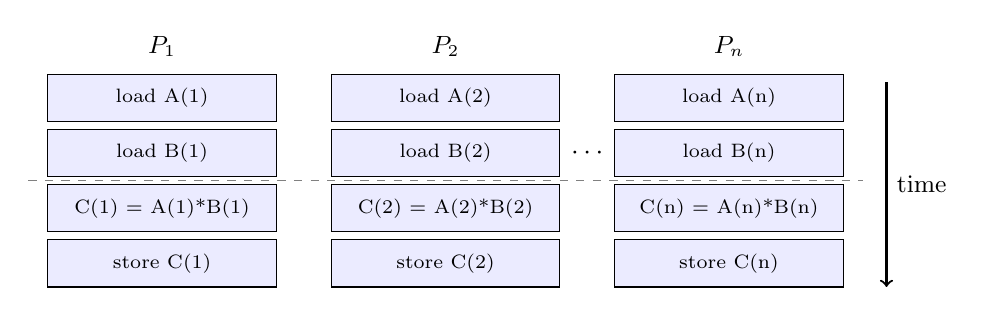
\begin{tikzpicture}[bx/.style={draw,minimum width=2.9cm,minimum height=6mm,font=\scriptsize,fill=blue!8}]
  \foreach \x/\lab/\i in {0/{$P_1$}/1, 3.6/{$P_2$}/2, 7.2/{$P_n$}/n} {
     \node[bx] at (\x,0)    {load \cl{A(\i)}};
     \node[bx] at (\x,-0.7) {load \cl{B(\i)}};
     \node[bx] at (\x,-1.4) {\cl{C(\i)} = \cl{A(\i)}*\cl{B(\i)}};
     \node[bx] at (\x,-2.1) {store \cl{C(\i)}};
     \node[font=\small\bfseries] at (\x,0.65) {\lab};
  }
  \node at (5.4,-0.7) {$\cdots$};
  \draw[->,thick] (9.2,0.2) -- (9.2,-2.4) node[midway,right,font=\small]{time};
  \draw[dashed,gray] (-1.7,-1.05) -- (8.9,-1.05);
\end{tikzpicture}
\end{center}

The dashed line illustrates lock-step: at the instant it marks, every element is in the same step.

\textbf{Where SIMD appears in real hardware.}
\begin{itemize}
  \item \emph{Vector processors} (Cray-90, Cray YMP in the slide): one instruction operates on a whole
        \emph{vector register} of numbers.
  \item \emph{Processor arrays} (the Connection Machine CM-2): thousands of simple processing
        elements under one control unit.
  \item \emph{SIMD instructions in today's CPUs}: SSE and AVX instructions process several numbers per
        instruction. An AVX-512 register is 512 bits wide and holds eight 64-bit doubles, so one instruction
        performs eight additions. Compilers use these automatically when they can prove the loop iterations
        are independent. This is the topic of ``vectorisation'' in your Chapter~1, section~1.5.
  \item \emph{GPUs}: threads are executed in groups that run the same instruction together. This is covered in the many-core
        slides.
\end{itemize}

\begin{pitfall}
\textbf{Branches hurt SIMD.} Suppose a loop body is \cl{if (x[i] > 0) y[i] = f(x[i]); else y[i] = g(x[i]);}
and eight lanes process eight values at once. The lanes cannot go different ways, since there is only one instruction stream. The
hardware first executes the \cl{f} path with the lanes where the condition is false switched off (``masked''), then the \cl{g}
path with the other lanes masked. Both paths are executed, and the cost is the \emph{sum}. SIMD works best on regular,
branch-free code.
\end{pitfall}

\subsection{MISD: multiple instructions, one data stream}

Several processing elements execute \emph{different} instructions on the \emph{same} data. The slide
simply says ``not popular''. The few uses are in fault-tolerant systems, where several units compute the same
result in different ways and a vote decides the answer, so that a single faulty unit is outvoted. Some authors count
systolic arrays here; others do not. For this course MISD is a box in the table and little else.

\subsection{MIMD: multiple instructions, multiple data}

Every processing element has its own instruction stream and its own data, and they run
\emph{independently and asynchronously}. At the same moment, one may be multiplying vectors while another
sorts a list and a third waits for input:

\begin{center}
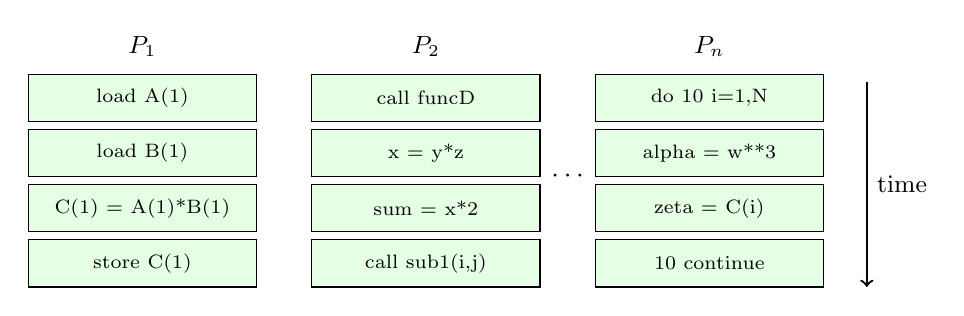
\begin{tikzpicture}[bx/.style={draw,minimum width=2.9cm,minimum height=6mm,font=\scriptsize,fill=green!10}]
  \node[font=\small\bfseries] at (0,0.65)   {$P_1$};
  \node[font=\small\bfseries] at (3.6,0.65) {$P_2$};
  \node[font=\small\bfseries] at (7.2,0.65) {$P_n$};
  \node[bx] at (0,0)    {load \cl{A(1)}};
  \node[bx] at (0,-0.7) {load \cl{B(1)}};
  \node[bx] at (0,-1.4) {\cl{C(1)} = \cl{A(1)}*\cl{B(1)}};
  \node[bx] at (0,-2.1) {store \cl{C(1)}};
  \node[bx] at (3.6,0)    {call \cl{funcD}};
  \node[bx] at (3.6,-0.7) {\cl{x = y*z}};
  \node[bx] at (3.6,-1.4) {\cl{sum = x*2}};
  \node[bx] at (3.6,-2.1) {call \cl{sub1(i,j)}};
  \node[bx] at (7.2,0)    {\cl{do 10 i=1,N}};
  \node[bx] at (7.2,-0.7) {\cl{alpha = w**3}};
  \node[bx] at (7.2,-1.4) {\cl{zeta = C(i)}};
  \node[bx] at (7.2,-2.1) {\cl{10 continue}};
  \node at (5.4,-1.0) {$\cdots$};
  \draw[->,thick] (9.2,0.2) -- (9.2,-2.4) node[midway,right,font=\small]{time};
\end{tikzpicture}
\end{center}

MIMD is the most general and by far the most common model: multicore laptops, clusters,
supercomputers (the slide's list: IBM SP, ``most other supercomputers, clusters, computational grids'').

\begin{intuition}
SIMD is a drill sergeant: every soldier does the same movement at the same moment. MIMD is a team of
workers, each with their own task list. SIMD is cheaper per unit of work when the task is regular; MIMD is
flexible enough for anything.
\end{intuition}

\paragraph{SPMD, a programming style (not a Flynn class).}
Most MPI programs are written as \term{SPMD}: Single Program, Multiple Data. Every process runs
\emph{the same program text}, but each uses its own identity (its \emph{rank}) to decide which part of the data to work on.
Because the processes run at their own pace and may take different branches, the hardware executing an SPMD program is MIMD,
\emph{not} SIMD. Do not confuse the two.

\begin{pitfall}
``A multicore CPU is SIMD'' is wrong. The \emph{cores} are independent, so the chip is MIMD. But \emph{inside each
core} there are SIMD units. Real machines combine both: MIMD across cores and SIMD within each core.
\end{pitfall}

\section{Classification by memory organisation}
\slides{5--7}

The second classification asks: when two processors want to exchange data, \emph{how do they do it}?
The answer depends on how memory is organised, and this choice shapes how parallel programs are written
more than any other. To state it precisely we first need the idea of an address space.

\subsection{Background: addresses and address spaces}

Memory can be pictured as a very long row of numbered boxes, one per byte. The box number is the
\term{address}. A pointer in C is just such a number. There are two kinds:
\begin{itemize}
  \item A \term{virtual address} is the number the \emph{program} uses. Each process sees its own private virtual
        address space, starting from zero. The operating system and hardware translate it.
  \item A \term{physical address} identifies an actual location in the DRAM chips.
\end{itemize}
Two different processes may both use the virtual address \cl{0x7FFF5FBFFD98} and refer to completely different
data, because their translations differ. This shows that the number alone means nothing until you also know \emph{whose} address space it
belongs to.

\begin{definition}{shared physical address space}
All processors address the same collection of memory locations: a given physical address refers to the \emph{same}
storage location no matter which processor uses it. If $P_1$ writes to that address, $P_2$
reading it sees the new value.
\end{definition}

\subsection{Shared-memory machines}

\begin{center}
\begin{tikzpicture}
  \foreach \i in {1,2,3,4} { \node[pe] (p\i) at (\i*1.7,2.1) {$P_\i$}; }
  \node[busbar,minimum width=7.6cm] (ic) at (3.4*1.25+0.2,1.0) {interconnect};
  \node[mm,minimum width=7.6cm] (m) at (3.4*1.25+0.2,0) {main memory (one address space)};
  \foreach \i in {1,2,3,4} { \draw[lnk] (p\i) -- (p\i |- ic.north); }
  \draw[lnk] (ic) -- (m);
\end{tikzpicture}
\end{center}

In a \term{shared-memory machine} all processors are connected to a common memory. Processors
communicate \emph{implicitly}: one writes a variable, another reads it, with ordinary loads and
stores. There are no explicit ``send'' operations. Programming is comparatively easy because data does not
have to be moved by hand, and the usual interface is \emph{threads} (OpenMP, pthreads). But it brings its own problems:

\begin{itemize}
  \item \textbf{Race conditions.} If two threads read and write the same location with no coordination, the result depends on
        timing. Take \cl{x = x + 1} executed by two threads, with \cl{x} initially $0$. The statement is really three steps
        (read \cl{x}, add one, write back):

  \begin{center}
  \begin{tabular}{@{}lll@{}}
  \toprule
  Step & Thread A & Thread B\\
  \midrule
  1 & read $x$ (gets $0$) & \\
  2 &  & read $x$ (gets $0$)\\
  3 & write $x=1$ & \\
  4 &  & write $x=1$\\
  \bottomrule
  \end{tabular}
  \end{center}
  Two increments were executed but $x=1$: one update was lost. Preventing this needs \emph{synchronisation}
  (locks, atomic operations), which later slides cover.
  \item \textbf{Cache coherence.} Each processor has its own cache holding \emph{copies} of memory.
        Keeping those copies consistent is a hardware problem (Chapter~3).
  \item \textbf{Contention.} Many processors using the same memory at once compete for its bandwidth.
\end{itemize}

\subsection{UMA and NUMA}

Shared-memory machines come in two kinds, depending on whether all memory is equally far from all processors.

\begin{center}
\begin{tikzpicture}[xscale=1.0]
  % UMA
  \node[font=\small\bfseries] at (1.6,3.5) {UMA};
  \node[pe] (a1) at (0,2.5) {$P_1$}; \node[pe] (a2) at (1.1,2.5) {$P_2$};
  \node[pe] (a3) at (2.2,2.5) {$P_3$}; \node[pe] (a4) at (3.3,2.5) {$P_4$};
  \node[busbar,minimum width=4.2cm] (ia) at (1.65,1.4) {interconnect};
  \node[mm,minimum width=4.2cm] (ma) at (1.65,0.4) {memory};
  \foreach \i in {1,2,3,4} \draw[lnk] (a\i) -- (a\i |- ia.north);
  \draw[lnk] (ia) -- (ma);
  % NUMA
  \node[font=\small\bfseries] at (8.6,3.5) {NUMA};
  \foreach \k/\x in {1/6.1,2/8.1,3/10.1} {
     \node[pe] (np\k) at (\x-0.45,2.5) {$P$}; \node[pe] (nq\k) at (\x+0.45,2.5) {$P$};
     \node[mm] (nm\k) at (\x,1.5) {mem};
     \draw[lnk] (np\k) -- (nm\k); \draw[lnk] (nq\k) -- (nm\k);
  }
  \node[busbar,minimum width=5.2cm] (ib) at (8.1,0.4) {interconnection network};
  \foreach \k in {1,2,3} \draw[lnk] (nm\k) -- (nm\k |- ib.north);
  \node at (9.15,2.0) {\large$\cdots$};
\end{tikzpicture}
\end{center}

\begin{definition}{UMA (Uniform Memory Access)}
Every processor needs the same time to access every memory location. These machines are also called
\emph{symmetric multiprocessors} (SMP). Data placement does not matter for performance.
\end{definition}

\begin{definition}{NUMA (Non-Uniform Memory Access)}
Memory is split into pieces attached to particular processors (or groups of them). A processor reaches
its \emph{local} memory quickly and \emph{remote} memory (attached to another processor) more slowly, but it is
\emph{still one shared address space}: the hardware carries out a remote load or store transparently. With coherent caches
this is called cc-NUMA.
\end{definition}

\textbf{Why does NUMA exist?} A single memory module, or a single bus to it, can only deliver a limited
bandwidth. If dozens of processors share it, it saturates. Attaching a piece of memory to each processor (or small group) multiplies the
total bandwidth with the number of processors, at the price of uneven access times. The machines named in
the slide (HP Exemplar, SGI Origin, Sequent NUMA-Q) are older examples. Today any multi-socket server is
NUMA: each socket has its own memory controller and DRAM, so a two-socket machine has two NUMA nodes. Remote
accesses typically cost noticeably more than local ones, often $1.5$ to $3$ times as much.

\begin{pitfall}
\textbf{NUMA is not distributed memory.} In NUMA a processor \emph{can} load from any memory in the machine
directly. In a distributed-memory machine (below) it cannot: the other node's memory is not in its address space.
\end{pitfall}

\textbf{What NUMA means for programmers.} The operating system normally places a memory page on the node of the thread that
\emph{first touches} it (the ``first-touch'' policy). If one thread initialises a huge array alone and then many threads on both sockets
process it, half the accesses become remote. Good NUMA code initialises data in parallel with the same distribution that
will later be used to compute on it. This is a performance issue only: the program is correct either way.

\subsection{Distributed-memory (message-passing) machines}

\begin{center}
\begin{tikzpicture}
  \foreach \i in {1,2,3,4} {
    \node[pe] (p\i) at (\i*1.7,2.1) {$P_\i$};
    \node[mm] (m\i) at (\i*1.7,1.1) {$M_\i$};
    \draw[lnk] (p\i) -- (m\i);
  }
  \node[busbar,minimum width=7.6cm] (ic) at (3.4*1.25+0.2,0) {interconnect};
  \foreach \i in {1,2,3,4} \draw[lnk] (m\i) -- (m\i |- ic.north);
\end{tikzpicture}
\end{center}

Here every processor has its \emph{own private memory} and there is no common address space. The processors can
exchange data only by sending \emph{messages} over the interconnect. If processor 1 wants a value that lives in
processor 2's memory, processor 2 must execute a \cl{send} and processor 1 a matching \cl{receive}. (Hence
the slide's alternative name, ``message-passing machine''.) Communication is \emph{explicit}.

\begin{itemize}
  \item \textbf{Advantages.} It scales to very large machines (thousands of nodes) because there is no need
        to keep caches coherent across the whole system, and it can be built from commodity nodes and a network.
  \item \textbf{Disadvantages.} The programmer must split the data among processors and manage every message.
        A message costs far more than a memory access (Chapter~4 gives a simple model). Programs are longer and
        harder to write; the standard interface is MPI.
\end{itemize}

\begin{pitfall}
In a distributed-memory program, sending a pointer to another process is meaningless: the address refers to
\emph{your} memory, not theirs. You must send the \emph{data} it points to.
\end{pitfall}

\subsection{Hybrid machines: what real systems look like}

Real supercomputers and clusters combine both models. Each \emph{node} is a small shared-memory (often NUMA) machine with many cores. The nodes are
connected into a distributed-memory machine by a network. Accelerators such as GPUs add yet another memory space
attached to a node. Programs correspondingly mix models, for example MPI between nodes and OpenMP threads within a node.

\begin{center}
\begin{tikzpicture}
  \foreach \k/\x in {1/0, 2/3.6, 3/7.2} {
    \node[draw,rounded corners,fill=gray!6,minimum width=3.0cm,minimum height=2.3cm] (nd\k) at (\x,1.0) {};
    \node[font=\scriptsize\bfseries] at (\x,1.95) {node \k};
    \foreach \c in {-1.05,-0.35,0.35,1.05} { \node[pe,minimum width=5.5mm,minimum height=5mm,font=\scriptsize] at (\x+\c,1.35) {c}; }
    \node[mm,minimum width=2.5cm] at (\x,0.65) {shared memory};
    \node[font=\scriptsize] at (\x,0.2) {(one address space per node)};
  }
  \node[busbar,minimum width=10.2cm] (net) at (3.6,-0.9) {network (message passing between nodes)};
  \foreach \x in {0,3.6,7.2} \draw[lnk] (\x,-0.15) -- (\x,-0.65);
\end{tikzpicture}
\end{center}

\subsection{Comparison}

\begin{center}
\small
\begin{tabularx}{\linewidth}{@{}l X X X@{}}
\toprule
 & \textbf{UMA} & \textbf{NUMA} & \textbf{Distributed memory}\\
\midrule
Address space & one, shared & one, shared & one \emph{per processor}\\
Access time & same for all memory & local fast, remote slower & local only; remote by message\\
Communication & implicit (loads/stores) & implicit (loads/stores) & explicit (send/receive)\\
Cache coherence hardware & yes & yes (cc-NUMA) & not across nodes\\
Typical programming & threads, OpenMP & threads, OpenMP (NUMA-aware) & MPI\\
Scalability & tens of processors & hundreds & thousands and more\\
\bottomrule
\end{tabularx}
\end{center}

\begin{keyidea}
The first classification (Flynn) says how the \emph{work} is organised; the second says how the \emph{memory} is organised. A modern
cluster is MIMD, and it is shared-memory inside each node and distributed-memory between nodes.
\end{keyidea}

\section*{Exercises}
\addcontentsline{toc}{section}{Exercises}
\begin{enumerate}[label=\textbf{\thechapter.\arabic*},leftmargin=*]
  \item Classify each as SISD, SIMD, MISD or MIMD: (a) an AVX instruction adding two vectors of eight doubles;
        (b) eight MPI processes each running the same program on a different part of an array; (c) a quad-core
        laptop running four different programs; (d) a single-core, single-threaded program.
  \item Two threads each execute \cl{x = x + 1} on a shared variable that starts at $0$. List all final values of
        $x$ that can occur, and explain how.
  \item Is a two-socket server with one memory bank per socket a shared-memory or a distributed-memory machine? Explain
        in two sentences what distinguishes it from a cluster of two single-socket servers.
  \item A \cl{for} loop over an array of 1000 elements uses AVX with 4 doubles per instruction. How many vector
        instructions does the loop need, ignoring loop overhead? What if the loop body contains a data-dependent
        \cl{if/else}?
  \item On a two-socket NUMA machine, thread~0 allocates and initialises a 2~GB array, then 16 threads
        (8 per socket) process it in parallel. Explain why this can be slower than expected and how to fix it.
\end{enumerate}